\section{Part B: Simulation Case Study}
\subsection{Topology and controller architecture}
The experiment uses four hosts and four Open vSwitch instances. The primary TCP pair is h1--h2; the optional competing UDP pair is h3--h4. Path A is s1--s2--s4, with two 10 Mbps, 5 ms core links. Path B is s1--s3--s4, with two 10 Mbps, 10 ms core links. Access links are 100 Mbps with 1 ms delay. The main comparison uses a 100-packet core queue verified using \texttt{tc}.

\begin{figure}[!htbp]\centering
\begin{tikzpicture}[x=1.25cm,y=1.15cm,every node/.style={font=\small},host/.style={draw,rounded corners,fill=blue!8,minimum width=1cm,minimum height=.5cm},sw/.style={draw,diamond,aspect=1.35,fill=gray!15,minimum width=.75cm,inner sep=1pt},flow/.style={-{Latex[length=2mm]},thick}]
% Keep both paths on separate horizontal lanes so link labels cannot collide.
\node[host] (h1) at (0,1.25) {h1};
\node[host] (h3) at (0,-1.25) {h3};
\node[sw] (s1) at (2,0) {s1};
\node[sw] (s2) at (4,1.25) {s2};
\node[sw] (s3) at (4,-1.25) {s3};
\node[sw] (s4) at (6,0) {s4};
\node[host] (h2) at (8,1.25) {h2};
\node[host] (h4) at (8,-1.25) {h4};
\draw[flow] (h1)--(s1);
\draw[flow] (h3)--(s1);
\draw[flow,blue] (s1)--node[midway,above,fill=white,inner sep=1pt,font=\scriptsize]{A: 10 Mbps, 5 ms}(s2);
\draw[flow,blue] (s2)--node[midway,above,fill=white,inner sep=1pt,font=\scriptsize]{10 Mbps, 5 ms}(s4);
\draw[flow,red] (s1)--node[midway,below,fill=white,inner sep=1pt,font=\scriptsize]{B: 10 Mbps, 10 ms}(s3);
\draw[flow,red] (s3)--node[midway,below,fill=white,inner sep=1pt,font=\scriptsize]{10 Mbps, 10 ms}(s4);
\draw[flow] (s4)--(h2);
\draw[flow] (s4)--(h4);
\end{tikzpicture}
\caption{Original vector topology diagram derived from the shared topology specification. Path A is blue and Path B is red.}
\label{fig:topology}
\end{figure}

\begin{figure}[htbp]\centering
\begin{tikzpicture}[node distance=.58cm,every node/.style={draw,rounded corners,align=center,fill=gray!10,minimum width=3.1cm,minimum height=.55cm,font=\small},>=Latex]
\node (counters) {OpenFlow port counters};
\node[below=of counters] (util) {Utilization from byte deltas};
\node[below=of util] (policy) {Static, B, or C policy};
\node[below=of policy] (rules) {Flow-rule updates};
\node[below=of rules] (outcomes) {Throughput, RTT, loss, and route events};
\draw[->] (counters)--(util); \draw[->] (util)--(policy); \draw[->] (policy)--(rules); \draw[->] (rules)--(outcomes);
\end{tikzpicture}
\caption{Controller measurement and decision pipeline.}
\label{fig:controller}
\end{figure}

\subsection{Policies and measurements}
Each path score is the maximum utilization of its two core egress links: s1:3 and s2:2 for A, and s1:4 and s3:2 for B. For each counter interval,
\[
U(\%) = \frac{\Delta\mathrm{tx\_bytes}\times8}{\Delta t\times\mathrm{capacity}_{bps}}\times100.
\]
Static retains its configured path. Policy B selects a measurably lower score; Policy C additionally requires a 15 percentage-point improvement and a 5,000 ms minimum dwell in the frozen reference configuration. The M5 poll interval is 1,000 ms.

E1 has no UDP competitor. E2 adds sustained 5 or 9 Mbps UDP on Path A. E3 uses three five-second 9 Mbps bursts beginning at 5, 15, and 25 seconds of a 30-second TCP run and declares C sensitivity variants. E4 disables s2--s4 one second into a 15-second run. Receiver-side iperf3 supplies TCP throughput; ping supplies RTT/loss; OpenFlow counters supply utilization.

\subsection{Results}
The completed campaign m5\_campaign\_20261011T115819Z contains 110 planned and recorded rows: 105 \texttt{ok}, five \texttt{failed}, and no aborted/excluded rows. The five failed rows are the expected static E4 outage controls. Processed 95\% Student-t intervals are descriptive; no significance test was performed.

\begin{figure}[htbp]\centering
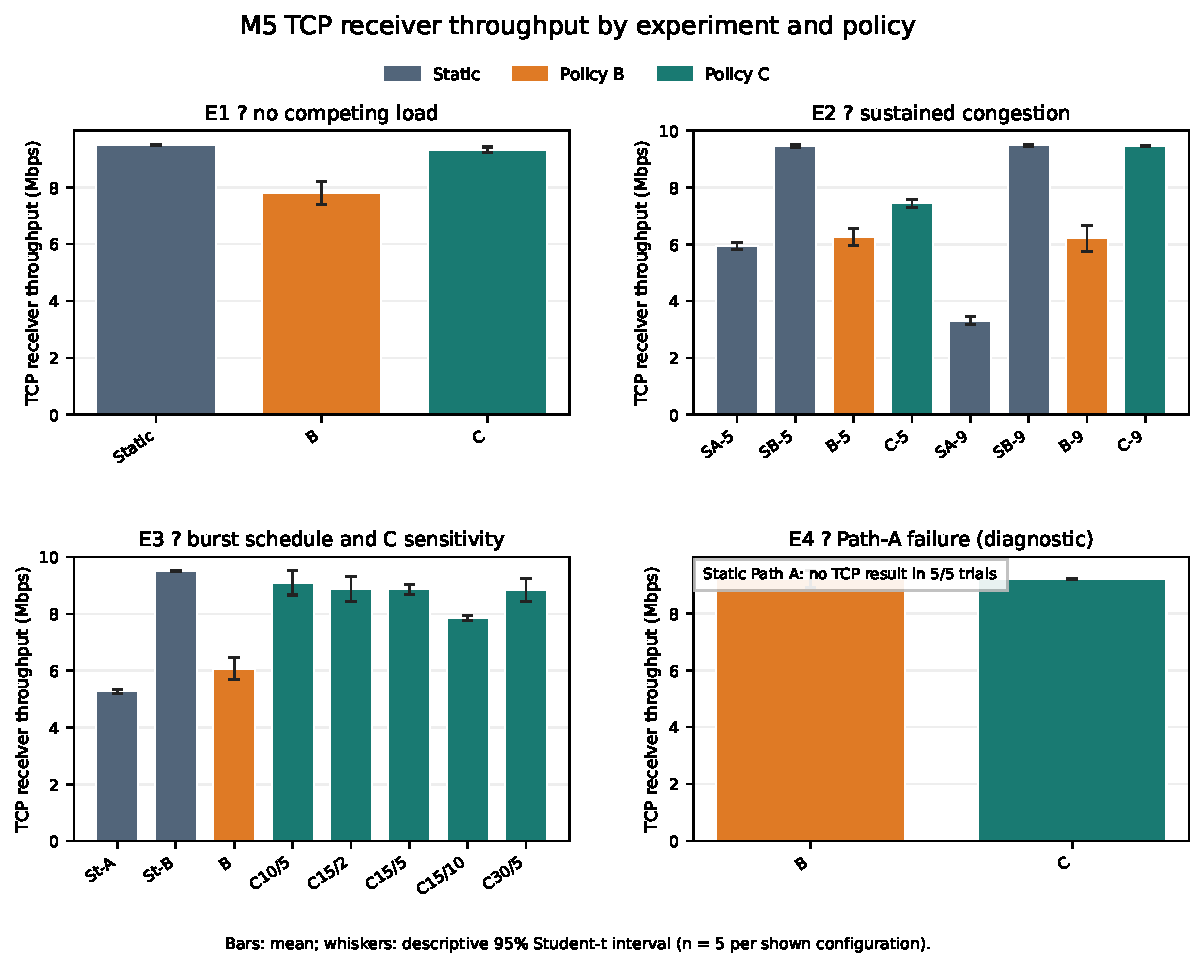
\includegraphics[width=.98\linewidth]{throughput_by_scenario.pdf}
\caption{TCP receiver throughput from the M5 processed summary. Bars show means and whiskers descriptive 95\% Student-t intervals. E2 labels are policy/load in Mbps (SA/SB denote Static on A/B); E3 C labels are margin points/dwell seconds. E4 Static on Path A has no TCP result in five outage trials.}
\label{fig:throughput}
\end{figure}

In E2 with 5 Mbps UDP, Static-on-A averaged 5.946 Mbps TCP receiver throughput, while Static-on-B averaged 9.465 Mbps (five trials each). In E1, B averaged 16 successful route changes per trial and C averaged three. E4 requires caution: B had already changed to Path B before the failure in all trials, while C was on A at failure and changed after it. Raw E4 switch-decision counts include rejected requests; successful route changes are taken from the event audit.

\begin{figure}[htbp]\centering
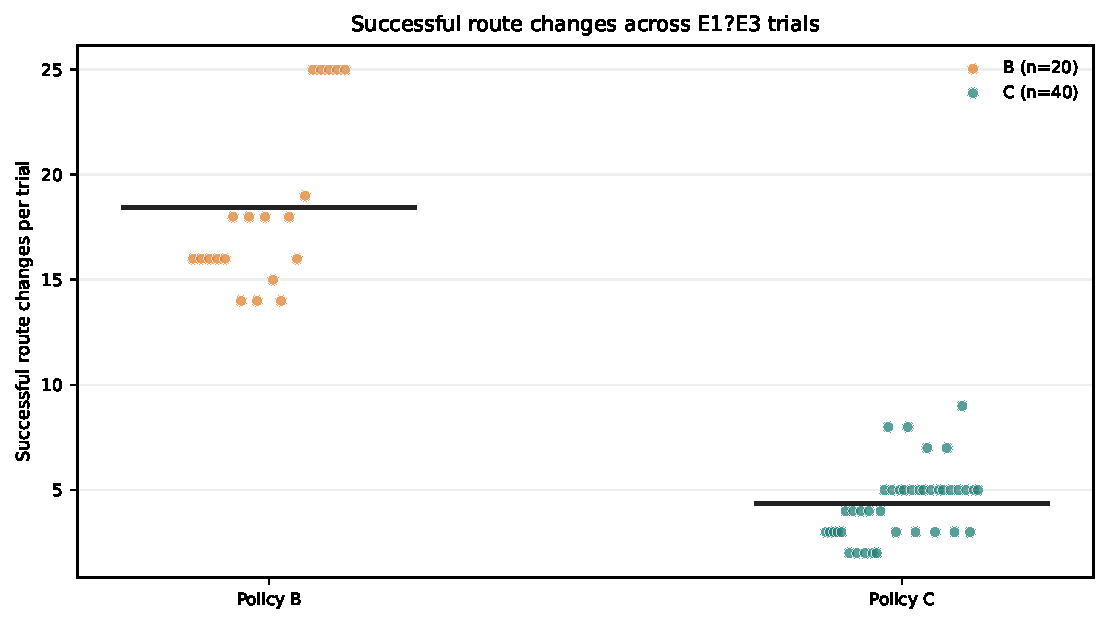
\includegraphics[width=.98\linewidth]{path_changes_b_vs_c.pdf}
\caption{Verified successful route-change comparison for E1--E3. E4 is excluded because its path state at failure differs by policy.}
\label{fig:changes}
\end{figure}

\begin{figure}[htbp]\centering
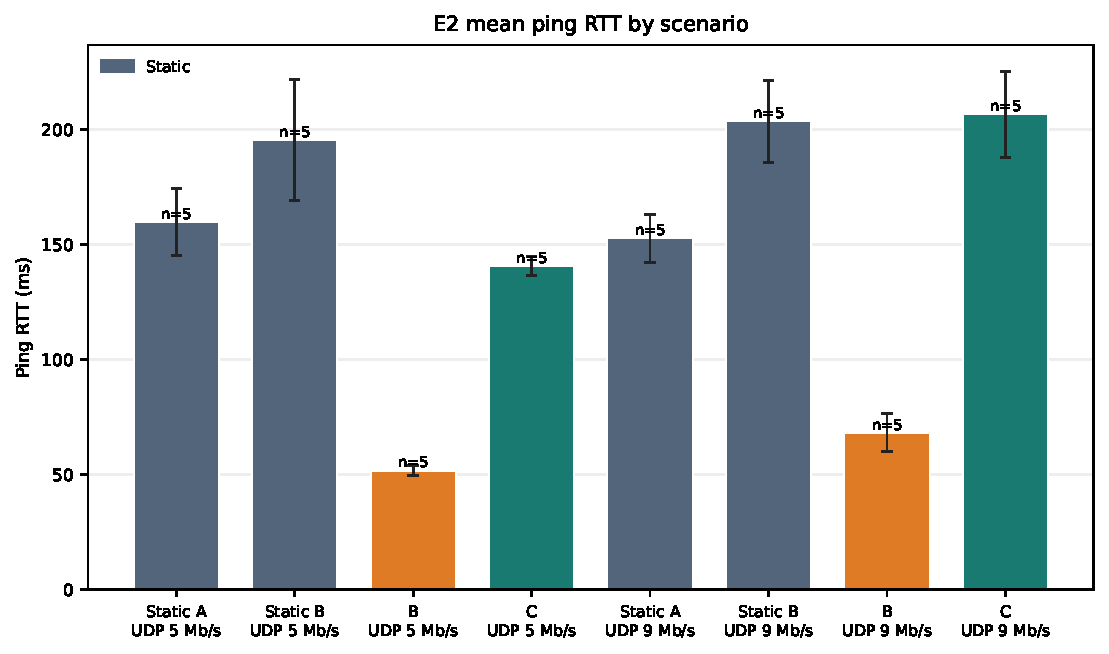
\includegraphics[width=.98\linewidth]{e2_rtt_mean.pdf}
\caption{Verified E2 mean ping-RTT figure. Latency and loss vary by scenario; no universal latency benefit is claimed.}
\label{fig:rtt}
\end{figure}

\begin{figure}[htbp]\centering
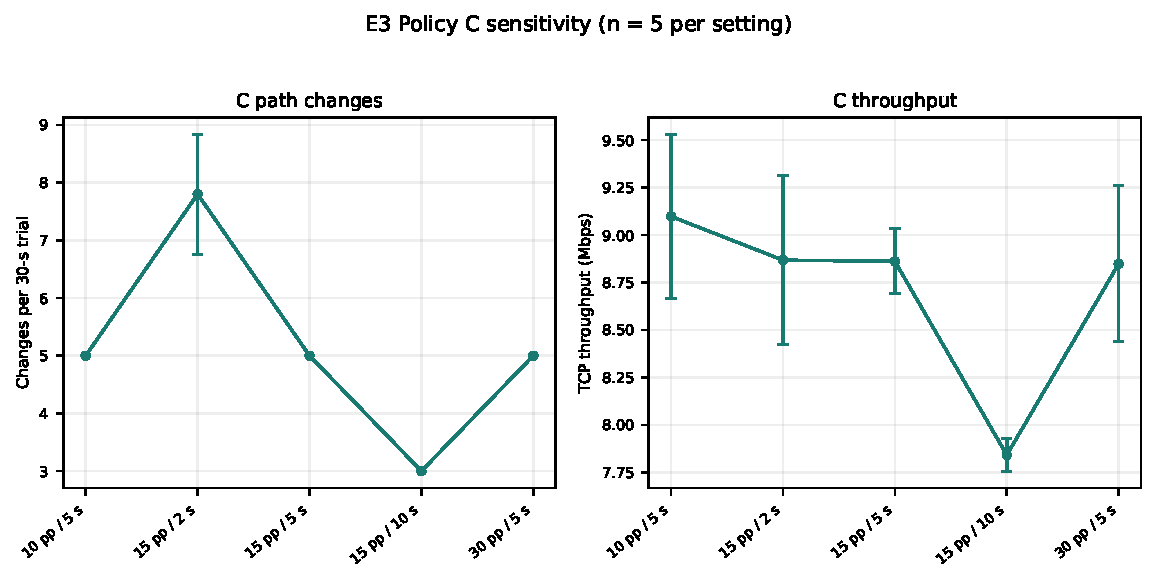
\includegraphics[width=.98\linewidth]{c_margin_dwell_sensitivity.pdf}
\caption{Verified E3 sensitivity figure for Policy C. The declared settings describe a trade-off and do not identify a universally best parameter pair.}
\label{fig:sensitivity}
\end{figure}

\begin{figure}[htbp]\centering
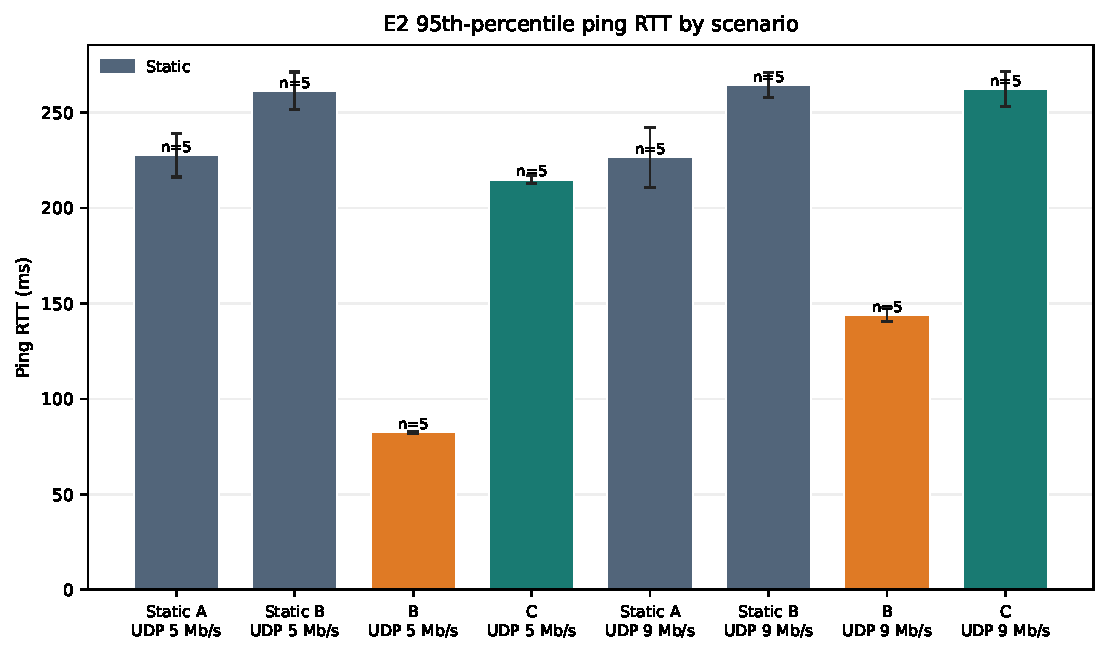
\includegraphics[width=.98\linewidth]{e2_rtt_p95.pdf}
\caption{E2 95th-percentile ping RTT from the processed campaign summary.}
\label{fig:rtt-p95}
\end{figure}

\begin{figure}[htbp]\centering
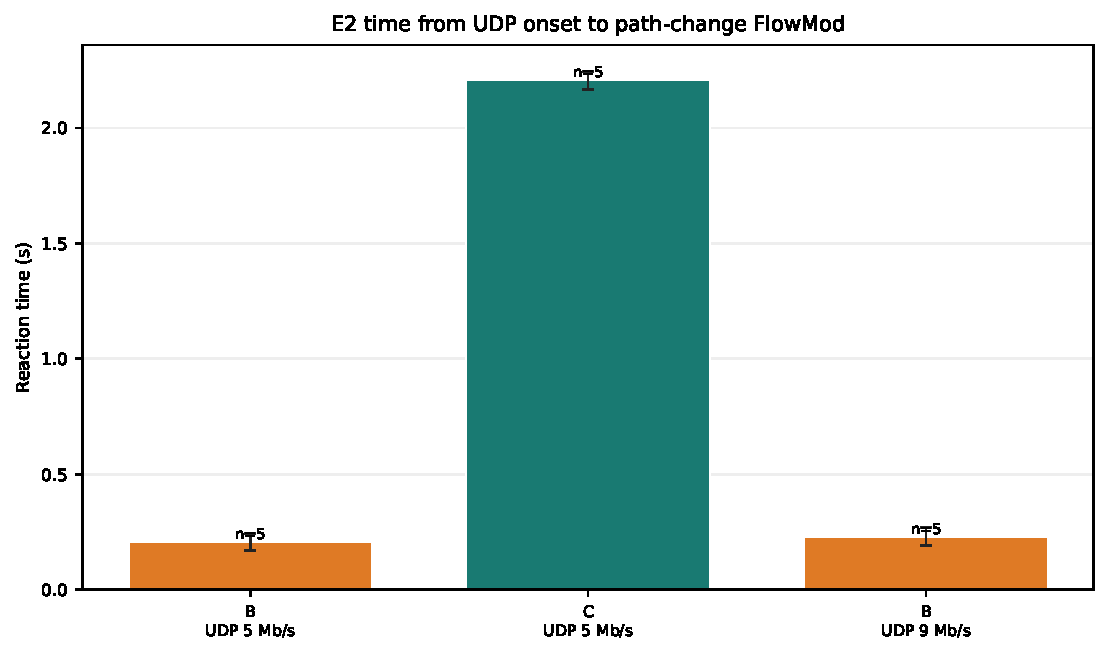
\includegraphics[width=.98\linewidth]{e2_reaction_time.pdf}
\caption{E2 time from UDP onset to the first route-change FlowMod. Empty cells indicate no qualifying event was recorded.}
\label{fig:reaction}
\end{figure}

The Static contrast isolates which path carries the competing flow. In E2 at 5 Mbps UDP, Static-on-A averaged 5.946 Mbps TCP, while Static-on-B averaged 9.465 Mbps (n=5 each); at 9 Mbps, the corresponding means were 3.311 and 9.482 Mbps. Values are rounded to three decimals from the M5 \texttt{metrics\_summary.csv} means (3.3114 and 9.4816 Mbps), grouped by scenario and algorithm.

\begin{table}[htbp]\centering
\caption{E2 static-path congestion contrast (M5 processed means; n=5).}
\label{tab:static-congestion}
\begin{tabular}{rrrr}
\toprule
UDP offered (Mbps) & Primary path & TCP receiver (Mbps) & Mean RTT (ms) \\
\midrule
5 & A & 5.946 & 159.86 \\
5 & B & 9.465 & 195.68 \\
9 & A & 3.311 & 152.75 \\
9 & B & 9.482 & 203.64 \\
\bottomrule
\end{tabular}
\end{table}

The source evidence PDF uses its own figure numbering, separate from the numbering generated in this report. Source evidence Figures 1--2 are live terminal captures; Figures 3--11 are archived evidence, including Figure 9, which is an archived M5 plot despite the PDF's erroneous opening note. Source Appendix Figures A1--A2 show earlier milestone validation, not M5 measurements.

\begin{figure}[htbp]\centering
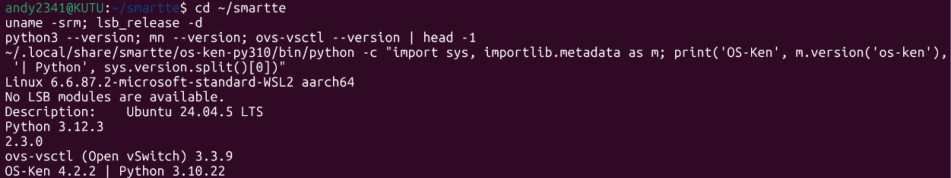
\includegraphics[width=.88\linewidth]{extracted/environment.png}
\caption{Live environment capture supplied by the team (source evidence Fig. 1). It records WSL2, Mininet, OVS, Python, and OS-Ken versions.}
\label{fig:evidence-environment}
\end{figure}

\begin{figure}[htbp]\centering
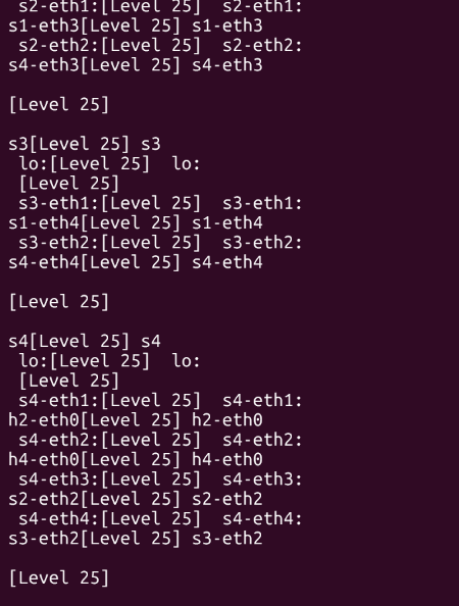
\includegraphics[width=.88\linewidth]{extracted/node_port_mapping.png}
\caption{Archived Mininet node and port listing (source evidence Fig. 3). This corroborates the host and switch port mapping used by the controller.}
\label{fig:evidence-ports}
\end{figure}

\begin{figure}[htbp]\centering
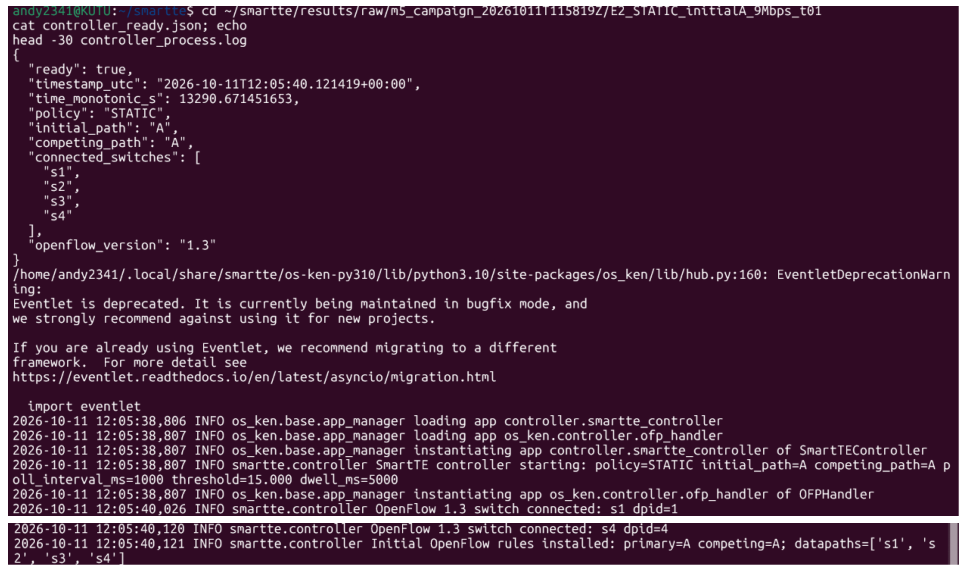
\includegraphics[width=.88\linewidth]{extracted/controller_startup_evidence.png}
\caption{Archived OS-Ken startup log from M5 trial E2\_STATIC\_initialA\_9Mbps\_t01 (source evidence Fig. 4); it shows the controller ready state and connected switches.}
\label{fig:evidence-controller}
\end{figure}

\paragraph{Queue configuration evidence.} The source evidence Fig. 7 is cropped and is not reproduced. The archived E2 static 9-Mbps trial's manifest and full per-interface \texttt{tc} output record \texttt{queue\_limit\_verified=true} and the 100-packet netem limit. This confirms the recorded configuration, not transient queue occupancy.

\begin{figure}[htbp]\centering
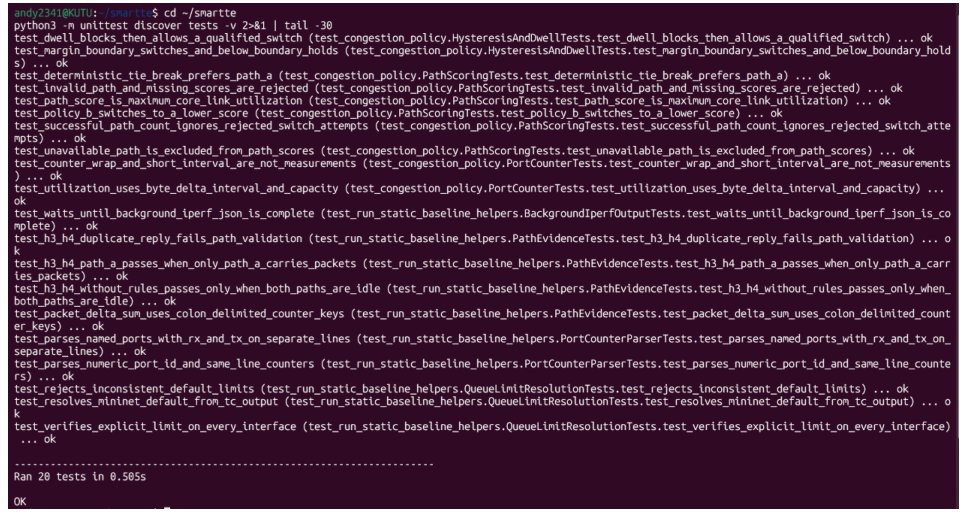
\includegraphics[width=.88\linewidth]{extracted/unit_tests_evidence.png}
\caption{Archived unit-test output showing 20 tests completed successfully (source evidence Fig. 8).}
\label{fig:evidence-tests}
\end{figure}

\begin{figure}[htbp]\centering
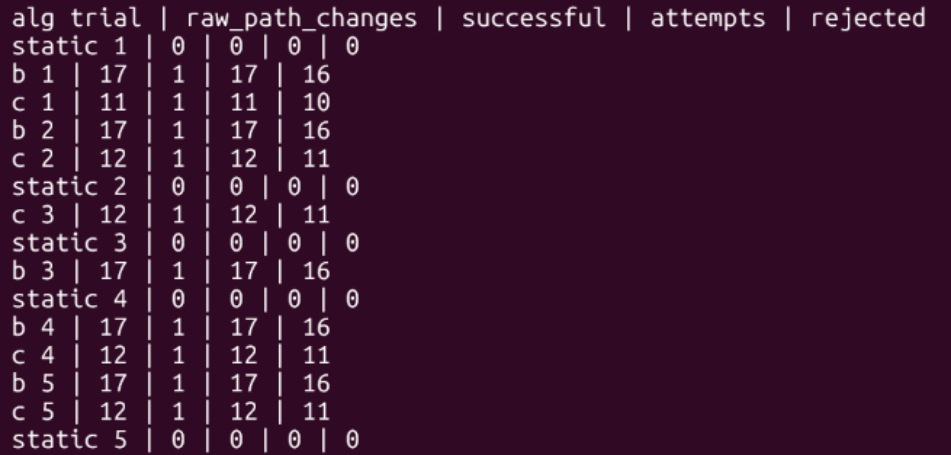
\includegraphics[width=.88\linewidth]{extracted/e4_path_change_audit_archived.png}
\caption{Archived E4 event audit (source evidence Fig. 11). It separates raw switch decisions from successful transitions and rejected attempts.}
\label{fig:evidence-e4}
\end{figure}

\subsection{E4 failure outcomes}
Table~\ref{tab:e4} separates policy outcome measures from controller decision counts. Successful transitions and decision attempts come from the processed event audit; recovery is counter-confirmed time after the link-down event.

\begin{table}[!htbp]\centering\small
\caption{E4 Path-A link-down outcomes (five trials per policy).}
\label{tab:e4}
\begin{tabular}{lccccc}
\toprule
Policy & \shortstack{TCP\\results} & \shortstack{Path B\\at failure} & \shortstack{Successful\\changes/trial} & \shortstack{Attempts\\per trial} & \shortstack{Rejected\\per trial} \\
\midrule
Static & 0/5 & 0/5 & 0 & 0 & 0 \\
B & 5/5 & 5/5 & 1 & 17 & 16 \\
C & 5/5 & 0/5 & 1 & 11.8 & 10.8 \\
\bottomrule
\end{tabular}

\smallskip
\begin{tabular}{lcc}
\toprule
Policy & \shortstack{Mean counter-confirmed\\recovery (s)} & \shortstack{Mean ping\\loss (\%)} \\
\midrule
Static & n/a & 93.33 \\
B & 0.193 & 2.13 \\
C & 1.005 & 1.87 \\
\bottomrule
\end{tabular}
\end{table}

The M5 metadata records campaign ID \texttt{m5\_20261011T115819Z}, commit \texttt{58acacd1\allowbreak20a1b8b8\allowbreak5b81d8a4\allowbreak6c1f2734\allowbreak79d18942}, and \texttt{git\_dirty=true}. The dirty flag means that commit alone does not identify the complete source state used during execution; the original metadata and trial evidence are preserved.

\subsection{Screenshot evidence}
The original seven-page evidence PDF is preserved at \texttt{evidence/SmartTE\_screenshots.pdf}; selected images were rasterized at 2x page resolution into \texttt{evidence/extracted/}. Source evidence Figures 2 (links) and 5 (static baseline) are not repeated because the vector topology and processed values communicate those details directly. The archived B-versus-C plot is Report Figure~\ref{fig:changes}. Source evidence Figures 1--2 are live terminal captures, Figures 3--11 are archived evidence, and Appendix Figures A1--A2 show earlier milestone validation. The opening provenance note's classification of source Figure 9 as live is incorrect; its caption identifies it as an archived plot.
